\documentclass[10pt,tikz,border=5pt]{standalone}
\usepackage{lmodern}
\usetikzlibrary{shapes.geometric}
\begin{document}
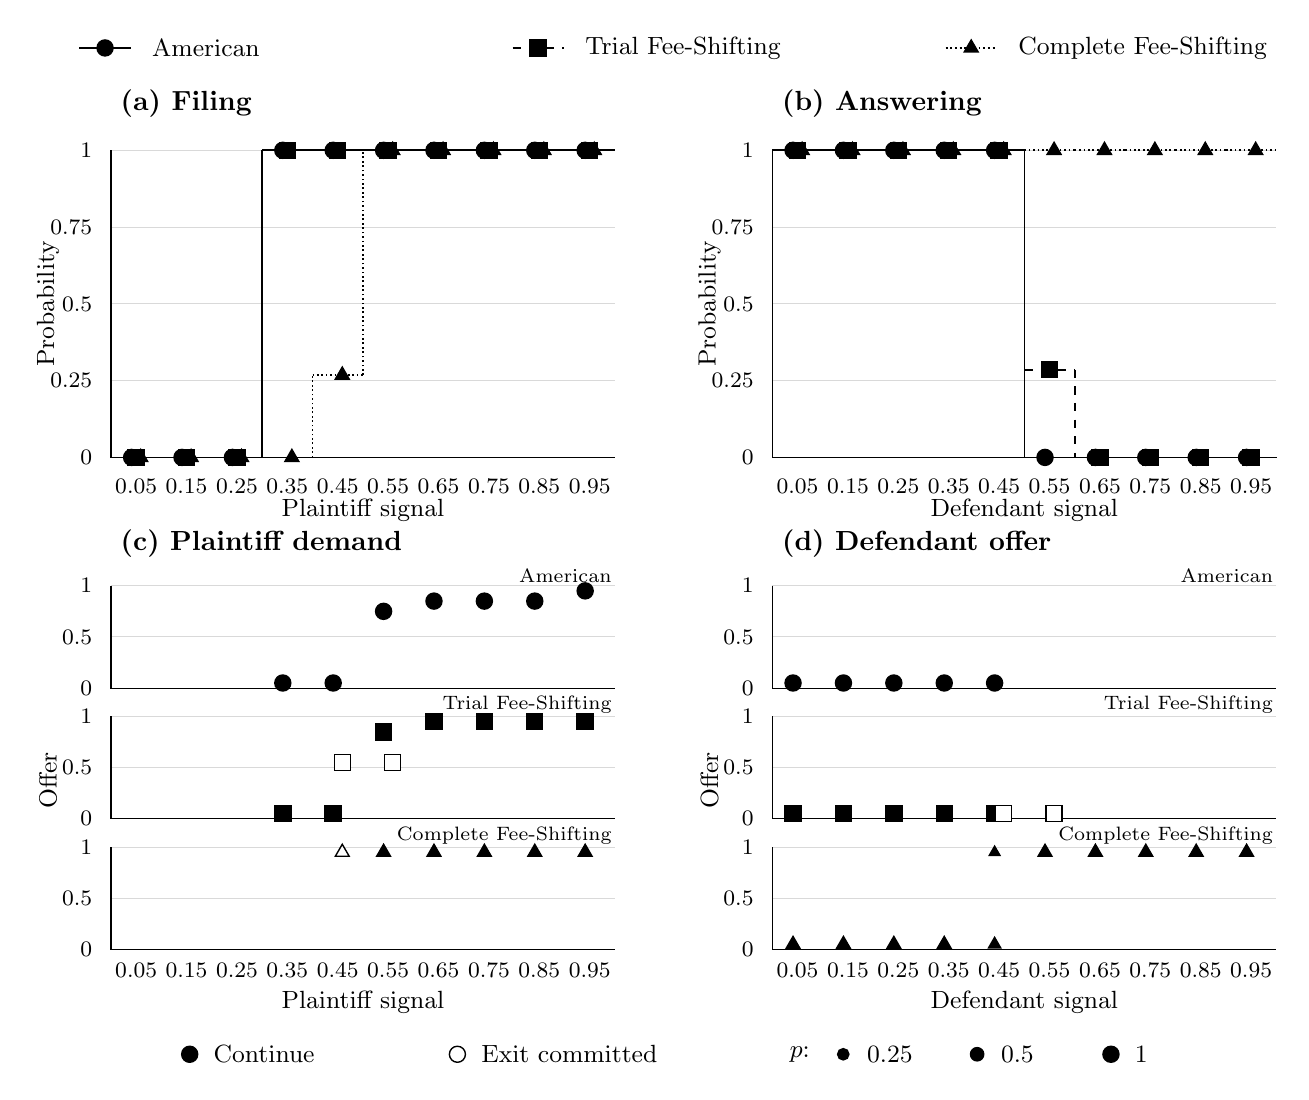
\begin{tikzpicture}[font=\small]\draw[solid,line width=.7pt] (0.6,12.3)--(1.25,12.3);
\node[draw=black,fill=black,circle,inner sep=0pt,minimum size=5.8pt,line width=.5pt] at (0.925,12.3) {};
\node[anchor=west] at (1.4,12.3) {American};
\draw[dashed,line width=.7pt] (6.1,12.3)--(6.75,12.3);
\node[draw=black,fill=black,rectangle,inner sep=0pt,minimum size=5.8pt,line width=.5pt] at (6.425,12.3) {};
\node[anchor=west] at (6.9,12.3) {Trial Fee-Shifting};
\draw[densely dotted,line width=.7pt] (11.6,12.3)--(12.25,12.3);
\node[draw=black,fill=black,regular polygon,regular polygon sides=3,inner sep=0pt,minimum size=5.8pt,line width=.5pt] at (11.925,12.3) {};
\node[anchor=west] at (12.4,12.3) {Complete Fee-Shifting};
\node[anchor=west,font=\bfseries] at (1,11.6) {(a) Filing};
\begin{scope}[shift={(1,7.1)},x=6.4cm,y=3.9cm]
\draw[black!15] (0,0)--(1,0);
\node[anchor=east,font=\footnotesize] at (-.018,0) {0};
\draw[black!15] (0,0.25)--(1,0.25);
\node[anchor=east,font=\footnotesize] at (-.018,0.25) {0.25};
\draw[black!15] (0,0.5)--(1,0.5);
\node[anchor=east,font=\footnotesize] at (-.018,0.5) {0.5};
\draw[black!15] (0,0.75)--(1,0.75);
\node[anchor=east,font=\footnotesize] at (-.018,0.75) {0.75};
\draw[black!15] (0,1)--(1,1);
\node[anchor=east,font=\footnotesize] at (-.018,1) {1};
\draw (0,1)--(0,0)--(1,0);
\node[anchor=north,font=\footnotesize] at (0.05,-.04) {0.05};
\node[anchor=north,font=\footnotesize] at (0.15,-.04) {0.15};
\node[anchor=north,font=\footnotesize] at (0.25,-.04) {0.25};
\node[anchor=north,font=\footnotesize] at (0.35,-.04) {0.35};
\node[anchor=north,font=\footnotesize] at (0.45,-.04) {0.45};
\node[anchor=north,font=\footnotesize] at (0.55,-.04) {0.55};
\node[anchor=north,font=\footnotesize] at (0.65,-.04) {0.65};
\node[anchor=north,font=\footnotesize] at (0.75,-.04) {0.75};
\node[anchor=north,font=\footnotesize] at (0.85,-.04) {0.85};
\node[anchor=north,font=\footnotesize] at (0.95,-.04) {0.95};
\draw[solid,line width=.6pt] (0,0)--(0.1,0);
\node[draw=black,fill=black,circle,inner sep=0pt,minimum size=5.8pt,line width=.5pt] at (0.041,0) {};
\draw[solid,line width=.6pt] (0.1,0)--(0.2,0);
\draw[solid,line width=.6pt] (0.1,0)--(0.1,0);
\node[draw=black,fill=black,circle,inner sep=0pt,minimum size=5.8pt,line width=.5pt] at (0.141,0) {};
\draw[solid,line width=.6pt] (0.2,0)--(0.3,0);
\draw[solid,line width=.6pt] (0.2,0)--(0.2,0);
\node[draw=black,fill=black,circle,inner sep=0pt,minimum size=5.8pt,line width=.5pt] at (0.241,0) {};
\draw[solid,line width=.6pt] (0.3,1)--(0.4,1);
\draw[solid,line width=.6pt] (0.3,0)--(0.3,1);
\node[draw=black,fill=black,circle,inner sep=0pt,minimum size=5.8pt,line width=.5pt] at (0.341,1) {};
\draw[solid,line width=.6pt] (0.4,1)--(0.5,1);
\draw[solid,line width=.6pt] (0.4,1)--(0.4,1);
\node[draw=black,fill=black,circle,inner sep=0pt,minimum size=5.8pt,line width=.5pt] at (0.441,1) {};
\draw[solid,line width=.6pt] (0.5,1)--(0.6,1);
\draw[solid,line width=.6pt] (0.5,1)--(0.5,1);
\node[draw=black,fill=black,circle,inner sep=0pt,minimum size=5.8pt,line width=.5pt] at (0.541,1) {};
\draw[solid,line width=.6pt] (0.6,1)--(0.7,1);
\draw[solid,line width=.6pt] (0.6,1)--(0.6,1);
\node[draw=black,fill=black,circle,inner sep=0pt,minimum size=5.8pt,line width=.5pt] at (0.641,1) {};
\draw[solid,line width=.6pt] (0.7,1)--(0.8,1);
\draw[solid,line width=.6pt] (0.7,1)--(0.7,1);
\node[draw=black,fill=black,circle,inner sep=0pt,minimum size=5.8pt,line width=.5pt] at (0.741,1) {};
\draw[solid,line width=.6pt] (0.8,1)--(0.9,1);
\draw[solid,line width=.6pt] (0.8,1)--(0.8,1);
\node[draw=black,fill=black,circle,inner sep=0pt,minimum size=5.8pt,line width=.5pt] at (0.841,1) {};
\draw[solid,line width=.6pt] (0.9,1)--(1,1);
\draw[solid,line width=.6pt] (0.9,1)--(0.9,1);
\node[draw=black,fill=black,circle,inner sep=0pt,minimum size=5.8pt,line width=.5pt] at (0.941,1) {};
\draw[dashed,line width=.6pt] (0,0)--(0.1,0);
\node[draw=black,fill=black,rectangle,inner sep=0pt,minimum size=5.8pt,line width=.5pt] at (0.05,0) {};
\draw[dashed,line width=.6pt] (0.1,0)--(0.2,0);
\draw[dashed,line width=.6pt] (0.1,0)--(0.1,0);
\node[draw=black,fill=black,rectangle,inner sep=0pt,minimum size=5.8pt,line width=.5pt] at (0.15,0) {};
\draw[dashed,line width=.6pt] (0.2,0)--(0.3,0);
\draw[dashed,line width=.6pt] (0.2,0)--(0.2,0);
\node[draw=black,fill=black,rectangle,inner sep=0pt,minimum size=5.8pt,line width=.5pt] at (0.25,0) {};
\draw[dashed,line width=.6pt] (0.3,1)--(0.4,1);
\draw[dashed,line width=.6pt] (0.3,0)--(0.3,1);
\node[draw=black,fill=black,rectangle,inner sep=0pt,minimum size=5.8pt,line width=.5pt] at (0.35,1) {};
\draw[dashed,line width=.6pt] (0.4,1)--(0.5,1);
\draw[dashed,line width=.6pt] (0.4,1)--(0.4,1);
\node[draw=black,fill=black,rectangle,inner sep=0pt,minimum size=5.8pt,line width=.5pt] at (0.45,1) {};
\draw[dashed,line width=.6pt] (0.5,1)--(0.6,1);
\draw[dashed,line width=.6pt] (0.5,1)--(0.5,1);
\node[draw=black,fill=black,rectangle,inner sep=0pt,minimum size=5.8pt,line width=.5pt] at (0.55,1) {};
\draw[dashed,line width=.6pt] (0.6,1)--(0.7,1);
\draw[dashed,line width=.6pt] (0.6,1)--(0.6,1);
\node[draw=black,fill=black,rectangle,inner sep=0pt,minimum size=5.8pt,line width=.5pt] at (0.65,1) {};
\draw[dashed,line width=.6pt] (0.7,1)--(0.8,1);
\draw[dashed,line width=.6pt] (0.7,1)--(0.7,1);
\node[draw=black,fill=black,rectangle,inner sep=0pt,minimum size=5.8pt,line width=.5pt] at (0.75,1) {};
\draw[dashed,line width=.6pt] (0.8,1)--(0.9,1);
\draw[dashed,line width=.6pt] (0.8,1)--(0.8,1);
\node[draw=black,fill=black,rectangle,inner sep=0pt,minimum size=5.8pt,line width=.5pt] at (0.85,1) {};
\draw[dashed,line width=.6pt] (0.9,1)--(1,1);
\draw[dashed,line width=.6pt] (0.9,1)--(0.9,1);
\node[draw=black,fill=black,rectangle,inner sep=0pt,minimum size=5.8pt,line width=.5pt] at (0.95,1) {};
\draw[densely dotted,line width=.6pt] (0,0)--(0.1,0);
\node[draw=black,fill=black,regular polygon,regular polygon sides=3,inner sep=0pt,minimum size=5.8pt,line width=.5pt] at (0.059,0) {};
\draw[densely dotted,line width=.6pt] (0.1,0)--(0.2,0);
\draw[densely dotted,line width=.6pt] (0.1,0)--(0.1,0);
\node[draw=black,fill=black,regular polygon,regular polygon sides=3,inner sep=0pt,minimum size=5.8pt,line width=.5pt] at (0.159,0) {};
\draw[densely dotted,line width=.6pt] (0.2,0)--(0.3,0);
\draw[densely dotted,line width=.6pt] (0.2,0)--(0.2,0);
\node[draw=black,fill=black,regular polygon,regular polygon sides=3,inner sep=0pt,minimum size=5.8pt,line width=.5pt] at (0.259,0) {};
\draw[densely dotted,line width=.6pt] (0.3,0)--(0.4,0);
\draw[densely dotted,line width=.6pt] (0.3,0)--(0.3,0);
\node[draw=black,fill=black,regular polygon,regular polygon sides=3,inner sep=0pt,minimum size=5.8pt,line width=.5pt] at (0.359,0) {};
\draw[densely dotted,line width=.6pt] (0.4,0.268097)--(0.5,0.268097);
\draw[densely dotted,line width=.6pt] (0.4,0)--(0.4,0.268097);
\node[draw=black,fill=black,regular polygon,regular polygon sides=3,inner sep=0pt,minimum size=5.8pt,line width=.5pt] at (0.459,0.268097) {};
\draw[densely dotted,line width=.6pt] (0.5,1)--(0.6,1);
\draw[densely dotted,line width=.6pt] (0.5,0.268097)--(0.5,1);
\node[draw=black,fill=black,regular polygon,regular polygon sides=3,inner sep=0pt,minimum size=5.8pt,line width=.5pt] at (0.559,1) {};
\draw[densely dotted,line width=.6pt] (0.6,1)--(0.7,1);
\draw[densely dotted,line width=.6pt] (0.6,1)--(0.6,1);
\node[draw=black,fill=black,regular polygon,regular polygon sides=3,inner sep=0pt,minimum size=5.8pt,line width=.5pt] at (0.659,1) {};
\draw[densely dotted,line width=.6pt] (0.7,1)--(0.8,1);
\draw[densely dotted,line width=.6pt] (0.7,1)--(0.7,1);
\node[draw=black,fill=black,regular polygon,regular polygon sides=3,inner sep=0pt,minimum size=5.8pt,line width=.5pt] at (0.759,1) {};
\draw[densely dotted,line width=.6pt] (0.8,1)--(0.9,1);
\draw[densely dotted,line width=.6pt] (0.8,1)--(0.8,1);
\node[draw=black,fill=black,regular polygon,regular polygon sides=3,inner sep=0pt,minimum size=5.8pt,line width=.5pt] at (0.859,1) {};
\draw[densely dotted,line width=.6pt] (0.9,1)--(1,1);
\draw[densely dotted,line width=.6pt] (0.9,1)--(0.9,1);
\node[draw=black,fill=black,regular polygon,regular polygon sides=3,inner sep=0pt,minimum size=5.8pt,line width=.5pt] at (0.959,1) {};
\end{scope}
\node at (4.2,6.43) {Plaintiff signal};
\node[rotate=90] at (0.2,9.05) {Probability};
\node[anchor=west,font=\bfseries] at (9.4,11.6) {(b) Answering};
\begin{scope}[shift={(9.4,7.1)},x=6.4cm,y=3.9cm]
\draw[black!15] (0,0)--(1,0);
\node[anchor=east,font=\footnotesize] at (-.018,0) {0};
\draw[black!15] (0,0.25)--(1,0.25);
\node[anchor=east,font=\footnotesize] at (-.018,0.25) {0.25};
\draw[black!15] (0,0.5)--(1,0.5);
\node[anchor=east,font=\footnotesize] at (-.018,0.5) {0.5};
\draw[black!15] (0,0.75)--(1,0.75);
\node[anchor=east,font=\footnotesize] at (-.018,0.75) {0.75};
\draw[black!15] (0,1)--(1,1);
\node[anchor=east,font=\footnotesize] at (-.018,1) {1};
\draw (0,1)--(0,0)--(1,0);
\node[anchor=north,font=\footnotesize] at (0.05,-.04) {0.05};
\node[anchor=north,font=\footnotesize] at (0.15,-.04) {0.15};
\node[anchor=north,font=\footnotesize] at (0.25,-.04) {0.25};
\node[anchor=north,font=\footnotesize] at (0.35,-.04) {0.35};
\node[anchor=north,font=\footnotesize] at (0.45,-.04) {0.45};
\node[anchor=north,font=\footnotesize] at (0.55,-.04) {0.55};
\node[anchor=north,font=\footnotesize] at (0.65,-.04) {0.65};
\node[anchor=north,font=\footnotesize] at (0.75,-.04) {0.75};
\node[anchor=north,font=\footnotesize] at (0.85,-.04) {0.85};
\node[anchor=north,font=\footnotesize] at (0.95,-.04) {0.95};
\draw[solid,line width=.6pt] (0,1)--(0.1,1);
\node[draw=black,fill=black,circle,inner sep=0pt,minimum size=5.8pt,line width=.5pt] at (0.041,1) {};
\draw[solid,line width=.6pt] (0.1,1)--(0.2,1);
\draw[solid,line width=.6pt] (0.1,1)--(0.1,1);
\node[draw=black,fill=black,circle,inner sep=0pt,minimum size=5.8pt,line width=.5pt] at (0.141,1) {};
\draw[solid,line width=.6pt] (0.2,1)--(0.3,1);
\draw[solid,line width=.6pt] (0.2,1)--(0.2,1);
\node[draw=black,fill=black,circle,inner sep=0pt,minimum size=5.8pt,line width=.5pt] at (0.241,1) {};
\draw[solid,line width=.6pt] (0.3,1)--(0.4,1);
\draw[solid,line width=.6pt] (0.3,1)--(0.3,1);
\node[draw=black,fill=black,circle,inner sep=0pt,minimum size=5.8pt,line width=.5pt] at (0.341,1) {};
\draw[solid,line width=.6pt] (0.4,1)--(0.5,1);
\draw[solid,line width=.6pt] (0.4,1)--(0.4,1);
\node[draw=black,fill=black,circle,inner sep=0pt,minimum size=5.8pt,line width=.5pt] at (0.441,1) {};
\draw[solid,line width=.6pt] (0.5,0)--(0.6,0);
\draw[solid,line width=.6pt] (0.5,1)--(0.5,0);
\node[draw=black,fill=black,circle,inner sep=0pt,minimum size=5.8pt,line width=.5pt] at (0.541,0) {};
\draw[solid,line width=.6pt] (0.6,0)--(0.7,0);
\draw[solid,line width=.6pt] (0.6,0)--(0.6,0);
\node[draw=black,fill=black,circle,inner sep=0pt,minimum size=5.8pt,line width=.5pt] at (0.641,0) {};
\draw[solid,line width=.6pt] (0.7,0)--(0.8,0);
\draw[solid,line width=.6pt] (0.7,0)--(0.7,0);
\node[draw=black,fill=black,circle,inner sep=0pt,minimum size=5.8pt,line width=.5pt] at (0.741,0) {};
\draw[solid,line width=.6pt] (0.8,0)--(0.9,0);
\draw[solid,line width=.6pt] (0.8,0)--(0.8,0);
\node[draw=black,fill=black,circle,inner sep=0pt,minimum size=5.8pt,line width=.5pt] at (0.841,0) {};
\draw[solid,line width=.6pt] (0.9,0)--(1,0);
\draw[solid,line width=.6pt] (0.9,0)--(0.9,0);
\node[draw=black,fill=black,circle,inner sep=0pt,minimum size=5.8pt,line width=.5pt] at (0.941,0) {};
\draw[dashed,line width=.6pt] (0,1)--(0.1,1);
\node[draw=black,fill=black,rectangle,inner sep=0pt,minimum size=5.8pt,line width=.5pt] at (0.05,1) {};
\draw[dashed,line width=.6pt] (0.1,1)--(0.2,1);
\draw[dashed,line width=.6pt] (0.1,1)--(0.1,1);
\node[draw=black,fill=black,rectangle,inner sep=0pt,minimum size=5.8pt,line width=.5pt] at (0.15,1) {};
\draw[dashed,line width=.6pt] (0.2,1)--(0.3,1);
\draw[dashed,line width=.6pt] (0.2,1)--(0.2,1);
\node[draw=black,fill=black,rectangle,inner sep=0pt,minimum size=5.8pt,line width=.5pt] at (0.25,1) {};
\draw[dashed,line width=.6pt] (0.3,1)--(0.4,1);
\draw[dashed,line width=.6pt] (0.3,1)--(0.3,1);
\node[draw=black,fill=black,rectangle,inner sep=0pt,minimum size=5.8pt,line width=.5pt] at (0.35,1) {};
\draw[dashed,line width=.6pt] (0.4,1)--(0.5,1);
\draw[dashed,line width=.6pt] (0.4,1)--(0.4,1);
\node[draw=black,fill=black,rectangle,inner sep=0pt,minimum size=5.8pt,line width=.5pt] at (0.45,1) {};
\draw[dashed,line width=.6pt] (0.5,0.285379)--(0.6,0.285379);
\draw[dashed,line width=.6pt] (0.5,1)--(0.5,0.285379);
\node[draw=black,fill=black,rectangle,inner sep=0pt,minimum size=5.8pt,line width=.5pt] at (0.55,0.285379) {};
\draw[dashed,line width=.6pt] (0.6,0)--(0.7,0);
\draw[dashed,line width=.6pt] (0.6,0.285379)--(0.6,0);
\node[draw=black,fill=black,rectangle,inner sep=0pt,minimum size=5.8pt,line width=.5pt] at (0.65,0) {};
\draw[dashed,line width=.6pt] (0.7,0)--(0.8,0);
\draw[dashed,line width=.6pt] (0.7,0)--(0.7,0);
\node[draw=black,fill=black,rectangle,inner sep=0pt,minimum size=5.8pt,line width=.5pt] at (0.75,0) {};
\draw[dashed,line width=.6pt] (0.8,0)--(0.9,0);
\draw[dashed,line width=.6pt] (0.8,0)--(0.8,0);
\node[draw=black,fill=black,rectangle,inner sep=0pt,minimum size=5.8pt,line width=.5pt] at (0.85,0) {};
\draw[dashed,line width=.6pt] (0.9,0)--(1,0);
\draw[dashed,line width=.6pt] (0.9,0)--(0.9,0);
\node[draw=black,fill=black,rectangle,inner sep=0pt,minimum size=5.8pt,line width=.5pt] at (0.95,0) {};
\draw[densely dotted,line width=.6pt] (0,1)--(0.1,1);
\node[draw=black,fill=black,regular polygon,regular polygon sides=3,inner sep=0pt,minimum size=5.8pt,line width=.5pt] at (0.059,1) {};
\draw[densely dotted,line width=.6pt] (0.1,1)--(0.2,1);
\draw[densely dotted,line width=.6pt] (0.1,1)--(0.1,1);
\node[draw=black,fill=black,regular polygon,regular polygon sides=3,inner sep=0pt,minimum size=5.8pt,line width=.5pt] at (0.159,1) {};
\draw[densely dotted,line width=.6pt] (0.2,1)--(0.3,1);
\draw[densely dotted,line width=.6pt] (0.2,1)--(0.2,1);
\node[draw=black,fill=black,regular polygon,regular polygon sides=3,inner sep=0pt,minimum size=5.8pt,line width=.5pt] at (0.259,1) {};
\draw[densely dotted,line width=.6pt] (0.3,1)--(0.4,1);
\draw[densely dotted,line width=.6pt] (0.3,1)--(0.3,1);
\node[draw=black,fill=black,regular polygon,regular polygon sides=3,inner sep=0pt,minimum size=5.8pt,line width=.5pt] at (0.359,1) {};
\draw[densely dotted,line width=.6pt] (0.4,1)--(0.5,1);
\draw[densely dotted,line width=.6pt] (0.4,1)--(0.4,1);
\node[draw=black,fill=black,regular polygon,regular polygon sides=3,inner sep=0pt,minimum size=5.8pt,line width=.5pt] at (0.459,1) {};
\draw[densely dotted,line width=.6pt] (0.5,1)--(0.6,1);
\draw[densely dotted,line width=.6pt] (0.5,1)--(0.5,1);
\node[draw=black,fill=black,regular polygon,regular polygon sides=3,inner sep=0pt,minimum size=5.8pt,line width=.5pt] at (0.559,1) {};
\draw[densely dotted,line width=.6pt] (0.6,1)--(0.7,1);
\draw[densely dotted,line width=.6pt] (0.6,1)--(0.6,1);
\node[draw=black,fill=black,regular polygon,regular polygon sides=3,inner sep=0pt,minimum size=5.8pt,line width=.5pt] at (0.659,1) {};
\draw[densely dotted,line width=.6pt] (0.7,1)--(0.8,1);
\draw[densely dotted,line width=.6pt] (0.7,1)--(0.7,1);
\node[draw=black,fill=black,regular polygon,regular polygon sides=3,inner sep=0pt,minimum size=5.8pt,line width=.5pt] at (0.759,1) {};
\draw[densely dotted,line width=.6pt] (0.8,1)--(0.9,1);
\draw[densely dotted,line width=.6pt] (0.8,1)--(0.8,1);
\node[draw=black,fill=black,regular polygon,regular polygon sides=3,inner sep=0pt,minimum size=5.8pt,line width=.5pt] at (0.859,1) {};
\draw[densely dotted,line width=.6pt] (0.9,1)--(1,1);
\draw[densely dotted,line width=.6pt] (0.9,1)--(0.9,1);
\node[draw=black,fill=black,regular polygon,regular polygon sides=3,inner sep=0pt,minimum size=5.8pt,line width=.5pt] at (0.959,1) {};
\end{scope}
\node at (12.6,6.43) {Defendant signal};
\node[rotate=90] at (8.6,9.05) {Probability};
\node[anchor=west,font=\bfseries] at (1,6.0) {(c) Plaintiff demand};
\begin{scope}[shift={(1,4.17)},x=6.4cm,y=1.3cm]
\draw[black!15] (0,0)--(1,0);
\node[anchor=east,font=\footnotesize] at (-.018,0) {0};
\draw[black!15] (0,0.5)--(1,0.5);
\node[anchor=east,font=\footnotesize] at (-.018,0.5) {0.5};
\draw[black!15] (0,1)--(1,1);
\node[anchor=east,font=\footnotesize] at (-.018,1) {1};
\draw (0,1)--(0,0)--(1,0);
\node[anchor=south east,font=\scriptsize,fill=white,inner sep=1pt] at (1,1) {American};
\node[draw=black,fill=black,circle,inner sep=0pt,minimum size=5.8pt,line width=.5pt] at (0.341,0.05) {};
\node[draw=black,fill=black,circle,inner sep=0pt,minimum size=5.8pt,line width=.5pt] at (0.441,0.05) {};
\node[draw=black,fill=black,circle,inner sep=0pt,minimum size=5.8pt,line width=.5pt] at (0.541,0.75) {};
\node[draw=black,fill=black,circle,inner sep=0pt,minimum size=5.8pt,line width=.5pt] at (0.641,0.85) {};
\node[draw=black,fill=black,circle,inner sep=0pt,minimum size=5.8pt,line width=.5pt] at (0.741,0.85) {};
\node[draw=black,fill=black,circle,inner sep=0pt,minimum size=5.8pt,line width=.5pt] at (0.841,0.85) {};
\node[draw=black,fill=black,circle,inner sep=0pt,minimum size=5.8pt,line width=.5pt] at (0.941,0.95) {};
\end{scope}
\begin{scope}[shift={(1,2.51)},x=6.4cm,y=1.3cm]
\draw[black!15] (0,0)--(1,0);
\node[anchor=east,font=\footnotesize] at (-.018,0) {0};
\draw[black!15] (0,0.5)--(1,0.5);
\node[anchor=east,font=\footnotesize] at (-.018,0.5) {0.5};
\draw[black!15] (0,1)--(1,1);
\node[anchor=east,font=\footnotesize] at (-.018,1) {1};
\draw (0,1)--(0,0)--(1,0);
\node[anchor=south east,font=\scriptsize,fill=white,inner sep=1pt] at (1,1) {Trial Fee-Shifting};
\node[draw=black,fill=black,rectangle,inner sep=0pt,minimum size=5.8pt,line width=.5pt] at (0.341,0.05) {};
\node[draw=black,fill=black,rectangle,inner sep=0pt,minimum size=5.8pt,line width=.5pt] at (0.441,0.05) {};
\node[draw=black,fill=black,rectangle,inner sep=0pt,minimum size=5.8pt,line width=.5pt] at (0.541,0.85) {};
\node[draw=black,fill=black,rectangle,inner sep=0pt,minimum size=5.8pt,line width=.5pt] at (0.641,0.95) {};
\node[draw=black,fill=black,rectangle,inner sep=0pt,minimum size=5.8pt,line width=.5pt] at (0.741,0.95) {};
\node[draw=black,fill=black,rectangle,inner sep=0pt,minimum size=5.8pt,line width=.5pt] at (0.841,0.95) {};
\node[draw=black,fill=black,rectangle,inner sep=0pt,minimum size=5.8pt,line width=.5pt] at (0.941,0.95) {};
\node[draw=black,fill=white,rectangle,inner sep=0pt,minimum size=5.8pt,line width=.5pt] at (0.459,0.55) {};
\node[draw=black,fill=white,rectangle,inner sep=0pt,minimum size=5.8pt,line width=.5pt] at (0.559,0.55) {};
\end{scope}
\begin{scope}[shift={(1,0.85)},x=6.4cm,y=1.3cm]
\draw[black!15] (0,0)--(1,0);
\node[anchor=east,font=\footnotesize] at (-.018,0) {0};
\draw[black!15] (0,0.5)--(1,0.5);
\node[anchor=east,font=\footnotesize] at (-.018,0.5) {0.5};
\draw[black!15] (0,1)--(1,1);
\node[anchor=east,font=\footnotesize] at (-.018,1) {1};
\draw (0,1)--(0,0)--(1,0);
\node[anchor=south east,font=\scriptsize,fill=white,inner sep=1pt] at (1,1) {Complete Fee-Shifting};
\node[anchor=north,font=\footnotesize] at (0.05,-.04) {0.05};
\node[anchor=north,font=\footnotesize] at (0.15,-.04) {0.15};
\node[anchor=north,font=\footnotesize] at (0.25,-.04) {0.25};
\node[anchor=north,font=\footnotesize] at (0.35,-.04) {0.35};
\node[anchor=north,font=\footnotesize] at (0.45,-.04) {0.45};
\node[anchor=north,font=\footnotesize] at (0.55,-.04) {0.55};
\node[anchor=north,font=\footnotesize] at (0.65,-.04) {0.65};
\node[anchor=north,font=\footnotesize] at (0.75,-.04) {0.75};
\node[anchor=north,font=\footnotesize] at (0.85,-.04) {0.85};
\node[anchor=north,font=\footnotesize] at (0.95,-.04) {0.95};
\node[draw=black,fill=black,regular polygon,regular polygon sides=3,inner sep=0pt,minimum size=5.8pt,line width=.5pt] at (0.541,0.95) {};
\node[draw=black,fill=black,regular polygon,regular polygon sides=3,inner sep=0pt,minimum size=5.8pt,line width=.5pt] at (0.641,0.95) {};
\node[draw=black,fill=black,regular polygon,regular polygon sides=3,inner sep=0pt,minimum size=5.8pt,line width=.5pt] at (0.741,0.95) {};
\node[draw=black,fill=black,regular polygon,regular polygon sides=3,inner sep=0pt,minimum size=5.8pt,line width=.5pt] at (0.841,0.95) {};
\node[draw=black,fill=black,regular polygon,regular polygon sides=3,inner sep=0pt,minimum size=5.8pt,line width=.5pt] at (0.941,0.95) {};
\node[draw=black,fill=white,regular polygon,regular polygon sides=3,inner sep=0pt,minimum size=5.8pt,line width=.5pt] at (0.459,0.95) {};
\end{scope}
\node at (4.2,.18) {Plaintiff signal};
\node[rotate=90] at (0.2,3.0) {Offer};
\node[anchor=west,font=\bfseries] at (9.4,6.0) {(d) Defendant offer};
\begin{scope}[shift={(9.4,4.17)},x=6.4cm,y=1.3cm]
\draw[black!15] (0,0)--(1,0);
\node[anchor=east,font=\footnotesize] at (-.018,0) {0};
\draw[black!15] (0,0.5)--(1,0.5);
\node[anchor=east,font=\footnotesize] at (-.018,0.5) {0.5};
\draw[black!15] (0,1)--(1,1);
\node[anchor=east,font=\footnotesize] at (-.018,1) {1};
\draw (0,1)--(0,0)--(1,0);
\node[anchor=south east,font=\scriptsize,fill=white,inner sep=1pt] at (1,1) {American};
\node[draw=black,fill=black,circle,inner sep=0pt,minimum size=5.8pt,line width=.5pt] at (0.041,0.05) {};
\node[draw=black,fill=black,circle,inner sep=0pt,minimum size=5.8pt,line width=.5pt] at (0.141,0.05) {};
\node[draw=black,fill=black,circle,inner sep=0pt,minimum size=5.8pt,line width=.5pt] at (0.241,0.05) {};
\node[draw=black,fill=black,circle,inner sep=0pt,minimum size=5.8pt,line width=.5pt] at (0.341,0.05) {};
\node[draw=black,fill=black,circle,inner sep=0pt,minimum size=5.8pt,line width=.5pt] at (0.441,0.05) {};
\end{scope}
\begin{scope}[shift={(9.4,2.51)},x=6.4cm,y=1.3cm]
\draw[black!15] (0,0)--(1,0);
\node[anchor=east,font=\footnotesize] at (-.018,0) {0};
\draw[black!15] (0,0.5)--(1,0.5);
\node[anchor=east,font=\footnotesize] at (-.018,0.5) {0.5};
\draw[black!15] (0,1)--(1,1);
\node[anchor=east,font=\footnotesize] at (-.018,1) {1};
\draw (0,1)--(0,0)--(1,0);
\node[anchor=south east,font=\scriptsize,fill=white,inner sep=1pt] at (1,1) {Trial Fee-Shifting};
\node[draw=black,fill=black,rectangle,inner sep=0pt,minimum size=5.8pt,line width=.5pt] at (0.041,0.05) {};
\node[draw=black,fill=black,rectangle,inner sep=0pt,minimum size=5.8pt,line width=.5pt] at (0.141,0.05) {};
\node[draw=black,fill=black,rectangle,inner sep=0pt,minimum size=5.8pt,line width=.5pt] at (0.241,0.05) {};
\node[draw=black,fill=black,rectangle,inner sep=0pt,minimum size=5.8pt,line width=.5pt] at (0.341,0.05) {};
\node[draw=black,fill=black,rectangle,inner sep=0pt,minimum size=5.8pt,line width=.5pt] at (0.441,0.05) {};
\node[draw=black,fill=white,rectangle,inner sep=0pt,minimum size=5.8pt,line width=.5pt] at (0.459,0.05) {};
\node[draw=black,fill=white,rectangle,inner sep=0pt,minimum size=5.8pt,line width=.5pt] at (0.559,0.05) {};
\end{scope}
\begin{scope}[shift={(9.4,0.85)},x=6.4cm,y=1.3cm]
\draw[black!15] (0,0)--(1,0);
\node[anchor=east,font=\footnotesize] at (-.018,0) {0};
\draw[black!15] (0,0.5)--(1,0.5);
\node[anchor=east,font=\footnotesize] at (-.018,0.5) {0.5};
\draw[black!15] (0,1)--(1,1);
\node[anchor=east,font=\footnotesize] at (-.018,1) {1};
\draw (0,1)--(0,0)--(1,0);
\node[anchor=south east,font=\scriptsize,fill=white,inner sep=1pt] at (1,1) {Complete Fee-Shifting};
\node[anchor=north,font=\footnotesize] at (0.05,-.04) {0.05};
\node[anchor=north,font=\footnotesize] at (0.15,-.04) {0.15};
\node[anchor=north,font=\footnotesize] at (0.25,-.04) {0.25};
\node[anchor=north,font=\footnotesize] at (0.35,-.04) {0.35};
\node[anchor=north,font=\footnotesize] at (0.45,-.04) {0.45};
\node[anchor=north,font=\footnotesize] at (0.55,-.04) {0.55};
\node[anchor=north,font=\footnotesize] at (0.65,-.04) {0.65};
\node[anchor=north,font=\footnotesize] at (0.75,-.04) {0.75};
\node[anchor=north,font=\footnotesize] at (0.85,-.04) {0.85};
\node[anchor=north,font=\footnotesize] at (0.95,-.04) {0.95};
\node[draw=black,fill=black,regular polygon,regular polygon sides=3,inner sep=0pt,minimum size=5.8pt,line width=.5pt] at (0.041,0.05) {};
\node[draw=black,fill=black,regular polygon,regular polygon sides=3,inner sep=0pt,minimum size=5.8pt,line width=.5pt] at (0.141,0.05) {};
\node[draw=black,fill=black,regular polygon,regular polygon sides=3,inner sep=0pt,minimum size=5.8pt,line width=.5pt] at (0.241,0.05) {};
\node[draw=black,fill=black,regular polygon,regular polygon sides=3,inner sep=0pt,minimum size=5.8pt,line width=.5pt] at (0.341,0.05) {};
\node[draw=black,fill=black,regular polygon,regular polygon sides=3,inner sep=0pt,minimum size=5.12334pt,line width=.5pt] at (0.441,0.05) {};
\node[draw=black,fill=black,regular polygon,regular polygon sides=3,inner sep=0pt,minimum size=4.435539pt,line width=.5pt] at (0.441,0.95) {};
\node[draw=black,fill=black,regular polygon,regular polygon sides=3,inner sep=0pt,minimum size=5.8pt,line width=.5pt] at (0.541,0.95) {};
\node[draw=black,fill=black,regular polygon,regular polygon sides=3,inner sep=0pt,minimum size=5.8pt,line width=.5pt] at (0.641,0.95) {};
\node[draw=black,fill=black,regular polygon,regular polygon sides=3,inner sep=0pt,minimum size=5.8pt,line width=.5pt] at (0.741,0.95) {};
\node[draw=black,fill=black,regular polygon,regular polygon sides=3,inner sep=0pt,minimum size=5.8pt,line width=.5pt] at (0.841,0.95) {};
\node[draw=black,fill=black,regular polygon,regular polygon sides=3,inner sep=0pt,minimum size=5.8pt,line width=.5pt] at (0.941,0.95) {};
\end{scope}
\node at (12.6,.18) {Defendant signal};
\node[rotate=90] at (8.6,3.0) {Offer};
\node[draw=black,fill=black,circle,inner sep=0pt,minimum size=5.8pt,line width=.5pt] at (2,-0.48) {};
\node[anchor=west] at (2.18,-.48) {Continue};
\node[draw=black,fill=white,circle,inner sep=0pt,minimum size=5.8pt,line width=.5pt] at (5.4,-0.48) {};
\node[anchor=west] at (5.58,-.48) {Exit committed};
\node[anchor=east] at (10,-.48) {$p$:};
\node[draw=black,fill=black,circle,inner sep=0pt,minimum size=4.1pt,line width=.5pt] at (10.3,-0.48) {};
\node[anchor=west] at (10.48,-.48) {0.25};
\node[draw=black,fill=black,circle,inner sep=0pt,minimum size=4.804163pt,line width=.5pt] at (12,-0.48) {};
\node[anchor=west] at (12.18,-.48) {0.5};
\node[draw=black,fill=black,circle,inner sep=0pt,minimum size=5.8pt,line width=.5pt] at (13.7,-0.48) {};
\node[anchor=west] at (13.88,-.48) {1};
\end{tikzpicture}
\end{document}
